% !TEX TS-program = pdflatex
\documentclass[11pt,a4paper,english]{article}
\usepackage[utf8]{inputenc}
\usepackage[T1]{fontenc}
\usepackage[obeyspaces, hyphens]{url}
\usepackage[top=4cm, bottom=4cm, left=3cm, right=3cm]{geometry}
\usepackage{enumerate}
\usepackage{amsmath}
\usepackage{mdwlist}
\usepackage{fancyhdr}
\usepackage{cite}
\usepackage{amsmath}
\usepackage[normalem]{ulem} % ulem enables strikethrough and more, but makes
                            % \emph underline by default :(
\usepackage{babel}
\usepackage{fancyvrb}
\usepackage{verbatimbox}
\usepackage{amsfonts}
\usepackage{amsthm}
%\usepackage{minted}
\usepackage{xcolor}
\usepackage{csquotes}
\usepackage{listings}
\usepackage{graphicx}
\usepackage{caption}
\usepackage{subcaption}
\usepackage{booktabs}
\usepackage{array}
\usepackage{lmodern} % better font
\usepackage[noend]{algpseudocode}
\usepackage{algorithm}
\usepackage{tikz}
\usepackage{paralist}
\usepackage[font=footnotesize,labelfont=bf]{caption}
\usetikzlibrary{arrows, decorations.markings}
\usepackage{hyperref} % always load hyper ref in the end
\usepackage{cleveref} % except cleveref
\newcolumntype{P}[1]{>{\centering\arraybackslash}p{#1}}

\newcommand*\justify{%
  \fontdimen2\font=0.4em% interword space
  \fontdimen3\font=0.2em% interword stretch
  \fontdimen4\font=0.1em% interword shrink
  \fontdimen7\font=0.1em% extra space
  \hyphenchar\font=`\-% allowing hyphenation
}

\lstset{
    frame=lrtb,
    captionpos=b,
    belowskip=0pt
}

\captionsetup[listing]{aboveskip=5pt,belowskip=\baselineskip}

\newcommand{\todo}[1]{\textcolor{red}{\textbf{TODO: }#1}}

%\definecolor{lightgray}{rgb}{0.95,0.95,0.95}
%\renewcommand\listingscaption{Code}

\newcommand{\concat}{\ensuremath{+\!\!\!\!+\!\!}}

\pagestyle{fancy}
\headheight 35pt

\DefineVerbatimEnvironment{code}{Verbatim}{fontsize=\small}
\DefineVerbatimEnvironment{example}{Verbatim}{fontsize=\small}
\newcommand{\ignore}[1]{}

\hyphenation{character-ised}

\rhead{Assignment 2}
\lhead{ACS}
\begin{document}

\thispagestyle{empty} %fjerner sidetal
\hspace{6cm} \vspace{6cm}
\begin{center}
\textbf{\Huge {Advanced Computer Systems}}\\ \vspace{0.5cm}
\Large{Assignment 2}
\end{center}
\vspace{3cm}
\begin{center}
\Large{\textbf{Truls Asheim, Rasmus Wriedt Larsen, Viktor Hansen}}
\end{center}
\vspace{6.0cm}
\thispagestyle{empty}

\newpage

\section{Exercises}

\subsection{Serializability \& Locking}

\subsubsection{Scenario 1}

\begin{figure}[H]
\centering
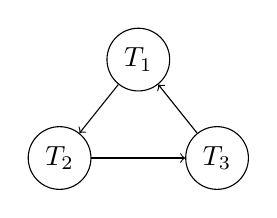
\begin{tikzpicture}
  \node[draw,circle] (t1) at (0,0) {$T_1$};
  \node[draw,circle] (t2) at (-1,-1.25) {$T_2$};
  \node[draw,circle] (t3) at (1,-1.25) {$T_3$};

  \draw [->] (t1) -- (t2);
  \draw [->] (t2) -- (t3);
  \draw [->] (t3) -- (t1);
\end{tikzpicture}
\end{figure}

%T1 precedes T2 (because of X)
%T2 precedes T3 (because of Z)
%T3 precedes T1 (because of Y)

As there is a cycle in the precedence graph, the schedule is \emph{not} conflict-serializable.

This schedule could not have been generated by strict two-phase locking
(non-conservative). The reason is \texttt{T1} will aquire a shared lock on
\texttt{X} initially, so \texttt{T2} will need to wait for \texttt{T1} to
commit, before it can get an exclusive lock on \texttt{X} for \texttt{W(X)}.

\subsubsection{Scenario 2}


\begin{figure}[H]
\centering
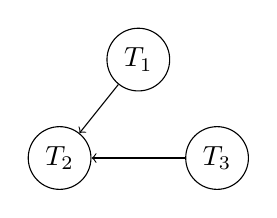
\begin{tikzpicture}
  \node[draw,circle] (t1) at (0,0) {$T_1$};
  \node[draw,circle] (t2) at (-1,-1.25) {$T_2$};
  \node[draw,circle] (t3) at (1,-1.25) {$T_3$};

  \draw [->] (t3) -- (t2);
  \draw [->] (t1) -- (t2);
\end{tikzpicture}
\end{figure}

%T3 precedes T2 (because of Z)
%T1 precedes T2 (because of Y and X)

As there is no cycles in the precedence graph, the schedule is conflict-serializable.

This schedule could be generated by strict two-phase locking (non-conservative),
as illustrated below.

\begin{verbatim}
T1: S(X)                            X(Y)  c
T2:                    S(Z)                       X(X) X(Y) C
T3:        X(Z)   C
\end{verbatim}

\subsection{Questions 2: Optimistic Concurrency Control}
In the Kung-Robinson optimistic concurrency model, we have to consider intersections of overlapping read and write sets, $R_{i}$ and $W_{i}$ respectively, for all transactions $T_{i}$. A non-empty intersection semantically corresponds to possible RAW, WAR and WAW conflicts/dependencies, i.e. if the same location is accessed by two different transactions and at least one of the accesses is a write. 


\paragraph{Scenario 1}
We will consider the intersection of all read and write sets that involve $T_{3}$, with a few restrictions. We know that (1) $T_{1}$ completes before $T_{3}$ begins with its write phase and (2) $T_{2}$ completes read phase before $T_{3}$ does. This means $R_{1} \cap W_{3} = \emptyset$, $W_{1} \cap R_{3} = \emptyset$, $W_{1} \cap W_{3} = \emptyset$ and $R_{2} \cap W_{3} = \emptyset$, $W_{2} \cap W_{3} = \emptyset$ as these read/write sets are guaranteed to not overlap. The intersections are depicted in Table \ref{tbl:scenario1}:
\begin{table}[!hbt]
\centering
\begin{tabular}{|c|c|c|c|}
\hline
$\cap$  & $W_{1}$ & $W_{2}$ & $W_{3}$    \\ \hline
$R_{1}$ & x  & x  & $\emptyset$ \\ \hline
$R_{2}$ & x  & x  & $\emptyset$ \\ \hline
$R_{3}$ & $\emptyset$ & $\left\{ 4 \right\}$ & x \\ \hline
$W_{1}$ & x  & x  & $\emptyset$ \\ \hline
$W_{2}$ & x  & x  & $\emptyset$ \\ \hline
$W_{3}$ & $\emptyset$ & $\emptyset$ & x \\ \hline
\end{tabular}
\caption{Intersections of all $R_{i}$ and $W_{i}$ that overlap and involve $T_{3}$.}
\label{tbl:scenario1}
\end{table}

In the case that $T_{2}$ writes element $4$ after $T_{3}$ has read element $4$, $T_{3}$ will have to perform a rollback, as RAW dependency is violated. In the case where $T_{2}$ writes element $4$ before $T_{3}$ reads element $4$, $T_{3}$ can commit.

\paragraph{Scenario 2} In this case, it is given that (1) $T_{1}$ completes before $T_{3}$ begins its write phase and (2) $T_{2}$ completes its read phase before $T_{3}$ begins its read phase. This means that $W_{1} \cap W_{3} = \emptyset$, $R_{1} \cap W_{3} = \emptyset$, $R_{2} \cap W_{3} = \emptyset$, 
\begin{table}[!hbt]
\centering
\begin{tabular}{|c|c|c|c|}
\hline
$\cap$  & $W_{1}$ & $W_{2}$ & $W_{3}$    \\ \hline
$R_{1}$ & x  & x  & $\emptyset$ \\ \hline
$R_{2}$ & x  & x  & $\emptyset$ \\ \hline
$R_{3}$ & $\left\{ 3 \right\}$ & $\emptyset$ & x \\ \hline
$W_{1}$ & x  & x  & $\emptyset$ \\ \hline
$W_{2}$ & x  & x  & $\emptyset$ \\ \hline
$W_{3}$ & $\emptyset$ & $\emptyset$ & x \\ \hline
\end{tabular}
\caption{Intersections of all $R_{i}$ and $W_{i}$ that overlap and involve $T_{3}$.}
\label{tbl:scenario1}
\end{table}

In the case, $T_{1}$ writes element $3$ after $T_{3}$ has read element $3$, $T_{3}$ will have to perform a rollback, as RAW dependency is violated. In the case where $T_{1}$ writes element $3$ before $T_{3}$ reads element $3$, $T_{3}$ can commit.

\paragraph{Scenario 3}
In this final case, we know that \begin{inparaenum}[1)] \item $T_1$ completes before
  $T_3$ starts its write phase and that \item $T_2$ completes before $T_3$
  starts its write phase \end{inparaenum}. All of the intersections between the
read and write sets can be seen in \Cref{tbl:scenario3}.

\begin{table}[!hbt]
\centering
\begin{tabular}{|c|c|c|c|}
\hline
$\cap$  & $W_{1}$ & $W_{2}$ & $W_{3}$    \\ \hline
$R_{1}$ & x  & x  & $\emptyset$ \\ \hline
$R_{2}$ & x  & x  & $\{7,8\}$ \\ \hline
$R_{3}$ & $\emptyset$ & $\emptyset$ & x \\ \hline
$W_{1}$ & x  & x  & $\emptyset$ \\ \hline
$W_{2}$ & x  & x  & $\emptyset$ \\ \hline
  $W_{3}$ & $\emptyset$ & $\emptyset$ & x \\ \hline
\end{tabular}
\caption{Intersections of all $R_{i}$ and $W_{i}$ that overlap and involve $T_{3}$.}
\label{tbl:scenario3}
\end{table}

As it can be seen, the only potential conflicts are between $R_2$ and $W_3$, but
since $T_2$ completes before $T_3$ starts its write phase its WAR dependency
isn't violated. Thus, $T_3$ can commit.

\section{Programming Assignments}
\subsection{Implementation}

\subsection{Questions for Concurrent Implementation of Bookstore}
\subsubsection{Description of Implementation}
\begin{enumerate}[(a)]
\item{Answer here!}
\item{Answer here!}
\end{enumerate}

\subsubsection{Correctness of Locking Protocol}
\subsubsection{Deadlock Occurrence}
\subsubsection{Scalability}
\subsubsection{Locking Overhead}


\end{document}

%%% Local Variables:
%%% mode: latex
%%% TeX-master: t
%%% End:
